\cotefile{67}
\scanpage{36}
\mspage{10}

\deleted{\unsure{et}}avec les pôles $0,\infty$. D'autre part, l'antipodisme $\sigma'z=-b/\bar z$ \deleted{transforme}\inserted{intervertit} $0$ et $\infty$, et \deleted{\unsure{pour} $z\in C$}\inserted{transforme} $C$ en lui-= car
\[
\begin{aligned}
z\in C&\quad\text{i.e.}\quad z\bar z=b\\
\text{implique}\quad \sigma'z\in C&\quad\text{i.e.}\quad
\underset{\underbrace{(-b/\bar z)(-b/z)}_{b^2/z\bar z}}{\underbrace{(\sigma'z)}\underbrace{\overline{(\sigma'z)}}}=b.
\end{aligned}
\]

Ainsi, $\sigma'$ et $(\sigma,\{0,\infty\})$ définissent la = structure riemannienne sphérique. On est content !

2) $N$ est ext \uline{non centrale} de $\gamma$ par $T$.

Cela signifie que si $\sigma\in N\setminus T$, on aura
\[
\sigma z=a\bar z,\quad\deleted{\unsure{\ne|1}}\quad(a\in\mathbb C^{\unsure{*|\times}}).
\]

\deleted{\unsure{D'où|Oui|Donc}}On en conclut
\[
\sigma^2z=a(\bar a z)=a\bar a z
\]
et la condition $\sigma^2\in T$ signifie
\[
a\bar a=1\quad\text{\deleted{\unsure{d.i.e.|i.e.|d'où}}}\quad a\in\mathbb U.
\]
qui implique aussi $\deleted{\sigma^2=1}$
\[
\sigma^2=1\qquad\text{i.e. l'extension $N$ est \uline{scindée}}
\]
\margin{Ici $N$ est déterminé en termes de $T$, i.e en termes de $\{z,z'\}$, comme $T\cup N^-$, où $N^-$ est formé de \uline{toutes} les anti-involutions de $X$ qui fixent $\{z,z'\}$. Donc il n'est pas question, des \unsure{élts seuls} de \unsure{not.}, d'extraire une métrique riem. sphérique}

Le produit $u_\theta\sigma$ $(\theta\in\mathbb U)$ est
\[
u_\theta\sigma(z)=(\theta a)\bar z\qquad\text{de la \deleted{\unsure{fo}} forme.}
\]
Soit $\alpha\inserted{\in\mathbb U}$ tel que
\[
a=\alpha^2=\alpha/\bar\alpha\qquad\text{donc}
\]
\[
z\in\mathbb C^\sigma\Longleftrightarrow z=\alpha\frac{\bar z}{\bar z}\Longleftrightarrow z/\unsure{a|\alpha}=\overline{(z/\alpha)}\quad\text{i.e.}\quad z\in\alpha\mathbb R
\]
% archive sheet number: 38
\scanpage{37}
\mspage{11}

En résumé et sauf erreur

\uline{Prop} Soit $X$ une sphère conforme \deleted{\unsure{orientée|marquée}}, $H\subset\mathrm{Aut}_{\mathrm{conf}}(X)\overset{\mathrm{déf}}=G$ un \deleted{\unsure{g}}sous-groupe \uline{compact} \deleted{de}, Alors

a) Il existe une métrique riemannienne sphérique normalisée sur $X$ comp. avec sa structure conforme

b) Celle-ci est unique sss \deleted{il n'existe pas de}\inserted{$X^H=\varnothing$}

\deleted{\unsure{pt}}\deleted{\unsure{b|c}}c) Supposons $\deleted{\unsure{X^H=|X^H\ne\varnothing}}$ $X^H\ne\varnothing$, $H\ne\{1\}$. Alors On a \deleted{\unsure{$X$}}\inserted{ou bien} $\operatorname{card}X^H=2$, ou bien $H=\{1,\sigma\}$ où $\sigma$ est une inversion.

1) Si $\operatorname{card}X^H=2$, \deleted{alors} $H\inserted{{}^+=H\cap G^+.\ \text{On a }X^H=X^{H^+},\ \text{et }H^+}$ est contenu dans un unique tore compact $T$, et \deleted{les \unsure{la structure|métriques sphériques}}\inserted{les métriques} sphériques riemanniennes normalisées comp., invariantes par \deleted{\unsure{$T$}} $H$, sont en corr. biunivoque avec les orbites de \inserted{$T$ dans} \deleted{(}$X\setminus X^H$\deleted{$)/T$} [donc tte orbite de \deleted{\unsure{$X$}} $H^+$ dans $X\setminus X^H$ définit une telle métrique]

% slanted
\margin{\uline{à vérifier} (\uline{NB} Il faudrait arriver à traduire en termes d'alg. linéaire, l'action d'un autom. \deleted{\unsure{de}} $\in G$ sur une métrique sphérique\ldots)}

\deleted{\unsure{d)|1')}} 2) Si $H=\{1,\sigma\}$, $\sigma$ une inversion, les métriques invariantes sous $H$ sont en corr. biunivoque avec les éléments de $(X\setminus X^H)/H=(X\setminus x^\sigma)/\sigma$
% archive sheet number: 39
\scanpage{38}
\mspage{12}

\uline{Récapitulation}

\deleted{A toute}\inserted{Soit $X$} surface conforme (sans bord), \deleted{\unsure{on peut|on peut lui},}\inserted{On peut} définir sur $X$ une métrique riemannienne canonique $Q_X$, \inserted{compatible avec str. conforme,} sauf dans les deux cas suivants :

a) $X\simeq\mathbb C$ \inserted{(i.e. $X$ droite affine sur un corps \inserted{top} $C$ isom. à $\mathbb C$)}, alors on peut définir quand même une classe de métriques riemanniennes compatibles, mod. multiplication par un scalaire. Ce sont les métriques stables par translation, qui sont aussi qu. inv. par tt autom. conforme de $X$. Elles sont \uline{plates} (donc : courbure nulle).

b) $X\simeq\mathbb P^1_{\mathbb C}$ (i.e $X$ droite projective sur un corps top $C$ \unsure{isom|$\mathbb R$-isom} à $\mathbb C$, ou encore $X$ sphère conforme). Alors il n'existe pas de métriques riemanniennes sur $X$ quasi-invariantes sous $G=\mathrm{Aut}\,X$, ni = sous $\mathrm{Aut}^+(X)$.

\deleted{Pour} Il y a pourtant sur $X$ un\deleted{e} \deleted{classe}\inserted{ens} can $R(X)$ de métriques riemanniennes (dites ``sphériques normalisées'') avec $\int_X dx=1$, qui forment une orbite sous $G$. Si $H\subset G$ est un sous-groupe, il existe un $Q\in R(X)$ stable par $H$ sss $H$ est rel cpt, et $Q$ est unique sss $X^H=\varnothing$. [Pour le cas $X^H\ne\varnothing$, cf proposition précédente qui détermine $R(x)^H$ dans tous les cas.]

% slanted
\margin{\uline{NB} $R(X)$ est un espace homogène de dim 3}
% archive sheet number: 40
\scanpage{39}
\mspage{13}

[NB \deleted{\unsure{Pour}}On pense notamment au cas où $X$ est associé à une \uline{carte}, et $H$ est le groupe des autom. de cette carte, qui est fini -- la condition $X^H=\varnothing$ signifie aussi qu'il n'y a pas de facette de la carte fixée par $H$...]

Dans tous les cas où $Q_X$ est défini, $Q_X$ est hyperbolique (i.e. : courbure $<0$) sss $X$ est hyperbolique, et alors $Q_X$ est de courbure \inserted{constante} égale à $-1$. D'autre part, $Q_X$ est \uline{plate} \deleted{dans les cas} (ou encore, à courbure nulle) sss $\widetilde X\simeq\mathbb C$ [y inclus le cas a) ci-dessus, où on a encore une $Q_X$ mod cte]. Le cas \unsure{restant|restreint} est celui du plan projectif réel, conforme, \deleted{qui est} \deleted{\unsure{dans le}}\inserted{pour} lequel $Q_X$ est une métrique homogène, de courbure Cte \deleted{égale à} et $>0$.

Donc chaque fois que $Q_X$ est défini, ou défini mod cte, il est à courbure constante, \deleted{\unsure{et est}} Il en est encore de = de $Q_{X,H}$ quand $X\simeq\mathbb P^1_{\mathbb C}$ et $H\subset\mathrm{Aut}_{\mathrm{conf}}X$ est cpt et tel que $X^H=\varnothing$, on trouve \deleted{une} métriques sph. euclidiennes, \unsure{donc|dans} de courbure constante $>0$.

% slanted
\margin{\uline{NB} Pour tte $X$ 0-connexe conforme, on \deleted{\illegible{1}} a dans l'ensemble \deleted{des métriques} $\mathrm{Riem}(X)$ des métr. riemanniennes comp. avec la str. conforme une orbite canonique sous $\mathrm{Aut}_{\mathrm{conf}}(X)$, qui est réduit à 1 pt dans tous les cas, sauf les cas a) et b) de la p. 12, où dans le cas a), on trouve une demi-droite dans $\mathrm{Riem}(X)$, et dans le cas b), une variété de dim 3 (\deleted{\unsure{qui|quelle}}\inserted{telle} \deleted{\unsure{les}} que $Q,Q'\in R(X)$ $Q\ne Q'$ implique $Q'$ et $Q$ \uline{non} prop.) Notion de métriques riemanniennes distinguées (a un sens aussi dans le cas \unsure{disconnexe|discontinu},}
% archive sheet number: 41
\scanpage{40}
\mspage{14}

\uline{Cas des surfaces conformes à bord} (pas néc. cptes)

On utilise l'équivalence de catégories
\[
\text{surfaces conformes à bord}\quad\overset{\sim}{\simeq}\quad
\begin{gathered}\text{surfaces holomorphes sans bord,}\\
\text{munies d'une antiinvolution.}\end{gathered}
\]
\diagram{\begin{tikzcd}[ampersand replacement=\&,row sep=small]
X \arrow[r,maps to] \& (X'=X^{\mathrm{or}},\sigma)\\
X=X'/\sigma \& (X',\sigma)\arrow[l,maps to]
\end{tikzcd}}

On dit que $X$ est hyperbolique sss $X^{\mathrm{or}}$ est hyperbolique \inserted{(i.e ses comp. connexes le sont)}

Quand $X$ est sans bord, on a $\widetilde X\simeq\widetilde{X^{\mathrm{or}}}$ (car $X^{\mathrm{or}}$ est un rev. étale de $X$) donc $X$ est hyperbolique au sens des réflexions précédentes, sss il l'est au nouveau sens.

Si $X$ est compact, \inserted{donc $X^{\mathrm{or}}$ aussi,} comme on a
\[
\chi(X^{\mathrm{or}})=2\chi(X)
\]
et que $\chi(X^{\mathrm{or}})<0\Longleftrightarrow X^{\mathrm{or}}\text{ hyperbolique}$, on trouve
\[
X\text{ hyperbolique}\Longleftrightarrow\chi(X)<0
\]

P.ex. si $X$ est holomorphe 0-connexe, de type $g,\unsure{\nu|v}$, cela signifie que $2g-2+\nu\geq1$ i.e $2g+\nu\geq3$

Mais on se gardera de confondre cette condition avec celle que $\mathrm{Int}\,X$ soit hyperbolique, ce qui est tjrs vrai sauf si $\nu=0$, $g\in\{0,1\}$..
% archive sheet number: 42
\scanpage{41}
\mspage{15}

Si $X$ est une surface conforme hyperbolique, alors la métrique canonique hyperbolique sur $X^{\mathrm{or}}$ se descend en une métrique hyperbolique sur $X$, pour laquelle le bord est géodésique.

Plus généralement, chaque fois que $X^{\mathrm{or}}$ est munie d'une métrique canonique, invariante par autom conformes [ou seulem$^{\mathrm t}$ par antiinvolutions, ce qui est le cas aussi si $X^{\mathrm{or}}\simeq\mathbb C$] alors celle-ci se descend à $X$, avec bord géodésique.

Quand $X$ est \deleted{\unsure{avec}}sans bord, \deleted{et \unsure{orientable|si elle}} alors \deleted{\unsure{la}} la métrique obtenue sur $X$ est celle déjà envisagée -- \deleted{\unsure{est}}\inserted{il y en a} dans tous les cas, sauf $X\simeq\mathbb P^1_{\mathbb C}$. On fera attention cependant que lorsque $X$ est le plan projectif réel, la deuxième prescription \deleted{\unsure{sans}} plus ne fournit\deleted{\unsure{s}} \uline{pas} de métrique -- elle le fait si on exige que la métrique sur $X^{\mathrm{or}}$ soit en $R(X^{\mathrm{or}})$, \uline{et} stable par $\sigma$ (ce qui la détermine sans ambiguïté). \deleted{De =}\inserted{\deleted{\unsure{De faç|De fait}}En sens inverse}, dans le cas $X\simeq\mathbb C$, $X^{\mathrm{or}}\simeq\mathbb C\amalg\mathbb C$, le procédé direct donne une classe de métriques (mod cte), la deuxième
% archive sheet number: 43
\scanpage{42}
\mspage{16}

ne donne quelque chose que si on la complète par la prescription que l'on prend une métrique ``distinguée'' sur $X^{\mathrm{or}}$ qui soit stable par $\sigma$.

Considérons maintenant les seuls cas nouveaux -- ceux où $X$ est 0-connexe et $\partial X\ne\varnothing$, correspondant à une $X^{\mathrm{or}}=\mathscr X$ connexe, munie d'une antiinvolution $\sigma$ telle que $\deleted{\unsure{\mathbb C}}\mathscr X^\sigma\ne\varnothing$. Les seuls cas problématiques pour l'existence d'une métrique canonique sur $X$, sont les suivants :

a') $\mathscr X\simeq\mathbb C$. \deleted{\unsure{Les anti.|Les aut.}}\inserted{OPS} $\mathscr X=\mathbb C$. Les anti-aut. de $\mathbb C$ sont
\[
z\longmapsto a\bar z+b\qquad(a\in\mathbb C^{\times},b\in\mathbb C)
\]
Si on prend une antiinvolution à pts fixes, OPS que $0$ est pt fixe, donc $b=0$, donc \deleted{l'application est $z\longmapsto a\bar z$}
\[
\sigma z=\deleted{\unsure{\alpha|a}}a\bar z\qquad\text{avec}\quad a\bar a=1\quad\text{i.e}\quad |a|=1\quad\text{i.e}\quad a\in\mathbb U
\]
(pour avoir $\sigma^2=\mathrm{id}$) soit

\deleted{l'ens des pts fixes est}
\[
\sigma z=\alpha^2\bar z=\alpha/\bar\alpha\,\bar z\qquad\text{si}\quad a=\alpha^2,\quad a\in\mathbb U,
\]
et l'ens des pts fixes est
\[
\mathbb C^\sigma=\alpha.\mathbb R
\]
\margin{symétrie p.r. à la droite $\alpha.\mathbb R$}
% archive sheet number: 44
\scanpage{43}
\mspage{17}

En fait, les antiinvolutions de $\mathbb C$ ont toutes des pts fixes, et ce sont les symétries orth. p.r. aux droites réelles (pas néc. passant par l'origine) \deleted{\unsure{par}}dans $\mathbb C$. La surface à bord conforme correspondante est isom. à un \uuline{demi-plan} (avec bord). On note que tte métrique \inserted{sur $\mathscr X$} quasi-invariante par autom. conforme, est invariante par autom d'ordre fini, en particulier par $\sigma$. Donc il y a sur $X$ une classe \inserted{can} de métriques riemanniennes, mod. cte.

\uline{NB} \deleted{\illegible{1}} Le modèle des $X$ envisagés est le demi-plan supérieur $\deleted{\unsure{\mathbb C|G}}$
\[
\overline{\mathbb H}=\{z\in\mathbb C\mid\unsure{\mathfrak I|\mathfrak J|\mathcal J}z\geq0\}.
\]
Le groupe des autom de $\overline{\mathbb H}$, isom au groupe des autom de la droite affine $\mathbb C$ qui commutent à $\sigma:z\longmapsto\bar z$, est \uline{le groupe affine réel}
% archive sheet number: 45
\scanpage{44}
\mspage{18}

b$'$) Cas $\mathscr X\simeq\mathbb P^1_{\mathbb C}$, $\sigma$ une inversion -- laquelle définit une structure de droite projective réelle -- on trouve \deleted{le disque} pour $X$ un \uline{disque}.

Pour obtenir une métrique distinguée sur $\mathscr X$ invariante par $\sigma$, il faut se donner un pt du disque ouvert $X\setminus\partial X$

\hfill\rule{0.34\linewidth}{0.4pt}\hfill\null

En résumé, tte surface conforme à bord $0$-connexe admet une unique métrique \deleted{\unsure{d}}Riemannienne distinguée, sauf dans les quatre cas suivants

a) a$'$) Cas $X\simeq\mathbb C$, ou $X\simeq\deleted{\unsure{\mathbb C}}\mathbb H=\{z\in\mathbb C\mathbin{/}\unsure{J|I|\mathfrak I}z\geq 0\}$ [droite affine complexe, demi plan à bord défini par une droite affine réelle], on a alors une classe de métriques mod constantes, qui forment une orbite sous $\mathrm{Aut}\, X$

b) b$'$) $X\simeq\mathbb P^1_{\mathbb C}$ ou $X\simeq\text{disque}$ [droite projective complexe ou \deleted{\unsure{demi espace projectif|demi plan projectif|droite projective}}\inserted{disque conforme} défini par droite projective réelle] -- il y a alors un ens. de métriques distinguées dépendant de 3 paramètres réels resp de 2 paramètres réels, également orbite sous $\mathrm{Aut}\,X$.

% archive sheet number: 46
\scanpage{45}
\mspage{\unsure{19|17|$1'$}}

\uline{Corollaire 3} Soit $\underset{\substack{\text{ouvert}\\\text{0-conn}}}{X\subset X'}$, $X'$ holo $0$-connexe

Alors $X$ est hyperbolique, sauf dans les cas suivants :

a) $X'$ est $\simeq\mathbb P^1_{\mathbb C}$ (resp $\mathbb E^1_{\mathbb C}$, resp. $\mathbb G_{m\,\mathbb C}$), et $\mathrm{Card}\,(X\setminus X')\leq 2$ (resp. $\leq 1$, resp. $=0$)

b) $X'$ est compacte de genre 1, et $X=X'$.

\uline{Remarque} Soit \deleted{\unsure{un|a}} $X$ une surface conforme $0$-connexe (pas néc. orientable). On dit encore que $X$ est hyperbolique si $\widetilde X\simeq\mathbb H$, ou ce qui revient au $=$, si tte \unsure{applic|applic.} conforme $\mathbb C\longrightarrow X$ est constante.

% slanted
\margin{ou encore si le rev. \deleted{\unsure{absol.|orienté|d'orient.}} \inserted{d'orientation} de $X$ (qui est une surface holomorphe,) est hyperbolique.}

Ainsi, les surfaces conformes \inserted{ss bord} $0$-connexes \uline{non} hyperboliques \unsure{sont|2 et}, en plus des quatre cas énumérés dans (i) ci-dessus, les quotients de telles surfaces par des antiinvolutions sans pts fixes. On trouve donc en plus

% archive sheet number: 47
\scanpage{46}
\mspage{21}

Dans le cas où $X$ est compacte, on trouve que c'est la seule métrique riemannienne (comp. avec la structure conforme) qui soit de courbure constante égale à $-1$.

2) Cas \deleted{elliptique} comp. et (orientable ou non) de genre 1. Dans le cas orienté, i.e. celui d'une courbe elliptique complexe, dont le rev. universel est une droite complexe, on a sur celui-ci une métrique canonique mod scalaires (métrique hermitienne) invariante par translations (et qu. inv. par tout autom i.e. par transformation affine), qu'on peut descendre \unsure{à|?|!} $X$. La constante multiplicative est

% archive sheet number: 48
\scanpage{48}
\mspage{\handwritten{1}}

% printed form
\deleted{J0369CNU}

\handwritten{15.1.}

\handwritten{$X$ \deleted{non singulière}\inserted{lisse type $g,\unsure{\nu|v}$} (sur $\overline{\mathbb Q}$)}

\handwritten{$Y$ stable non lisse type $(g,\nu)$ avec propagateur normal $N$, d'où un groupe fondamental \deleted{modifié}\inserted{ext.} $\pi_1\deleted{\unsure{\langle|(}}[Y,N\deleted{\unsure{\rangle|)}}]$.}

\handwritten{$X\underset{T}{\overset{\unsure{\varphi|f|\tau}}{\simeq}}Y$ un isomorphisme de Teichmüller.}

\handwritten{\uline{NB} Cet isomorphisme induit un isom de groupes extérieurs \deleted{\unsure{(et est dé|Ceci est de}} (et est déterminé par lui)
\[
\pi_1(X)\longrightarrow\pi_1(\deleted{\unsure{\langle|(}}[Y,N\deleted{\unsure{\rangle|)}}]).
\]}

\handwritten{\deleted{\unsure{On|O}}Quand on se donne un ``pt base sur $X$'' (ordinaire, ou à l'infini), et un sur $[Y,N]$ (idem -- et de plus distinct des pts singuliers de $Y$) on a une notion d'isom de Teichmüller \unsure{respectant|respect. nt} les pts marqués, \deleted{\unsure{et dét. un isom|et est un isom}}\inserted{(on suppose} qu'ils sont tous deux à distance finie, ou tous deux à l'infini) et on trouve alors un isom de groupes
\[
\text{(pas ext. !)}\qquad \pi_1(X,\unsure{x|\bullet})\longrightarrow\pi_1([Y,N],y)
\]}

\handwritten{En tout état de cause, \deleted{\unsure{l'iso|il}} l'isom extérieur déjà n'est pas compatible avec les actions ext. de $\mathrm{Gal}\,(\overline{\mathbb Q}/K)$, $K$ une \inserted{ss} extension finie de $\overline{\mathbb Q}/\mathbb Q$ assez grande.}

\handwritten{\uline{NB} Mettre en évidence \uline{trois} classes de conjugaison d'\deleted{éléments} hom. $\widehat{\mathbb Z}(1)\longrightarrow\pi_1(X)$ (deux seulement si $\nu\unsure{\geq|=|\ne|>}0$, l'une des trois étant les ``lacets'').}

% archive sheet number: 50
\scanpage{49}
\mspage{\handwritten{\unsure{$\sim$|2}}}

% printed form
\deleted{\texttt{/*JOB=CRAY2,ACCT=*********,ALL=M06,MSGL=N}\\
\texttt{// JOB MSGLEVEL=(1,1),MSGCLASS=A}\\
\texttt{// EXEC PGM=IEFBR14}}

\handwritten{\uline{A examiner} : a) Extension de la conjecture fondamentale en géom. alg. anabélienne aux courbes anabéliennes \deleted{\unsure{stabl|stab|stables}} singulières (stables, avec propagateur normal). \unsure{?|P}}

\handwritten{b) Pour une $Y$, anabélienne singulière donnée (sur corps $\deleted{\unsure{k}}K$ de t.f. sur $\mathbb Q$), \deleted{\unsure{On}}est-il vrai qu'on récupère les \unsure{él.|cl.} de \deleted{(pts}$\mathrm{Sing}(Y)$ $\cup$ $\underbrace{\text{Pts marqués}}_{Y_\infty}$ en termes des \inserted{classes de conj.} sous-groupes de $\pi_1(Y)$ isom. à $\widehat{\mathbb Z}$, et \unsure{esst|exst|ext.} normalisés par $\pi_1(K)$ (l'opération de $\pi_1(K)$ dessus se fera automatiquement via le caractère cyclotomique)}

\handwritten{c) S'inspirant des compactifications MD des $M_{g,\nu}$, définir ce que c'est qu'une compactification anabélienne d'une variété lisse anabélienne (sur un corps $K$ de car. 0, qu'on peut supposer être de type fini sur $\mathbb Q$). Comportement par spécialisation ???}

% archive sheet number: 51
\scanpage{50}
Générateurs et relations pour les groupoïdes et groupes de Teichmüller (spéciaux et ordinaires, évt. toriques...)

Je m'attends à trouver trois types de présentations, à propriétés complémentaires -- mais toutes à significations arithmétiques :

a) Présentation par ``pa\uline{ntalons}'' ou ``\uline{triades}''. Elle revient à travailler sur les pts à l'infini ``les plus critiques'' sur les multiplicités modulaires, et semble (d'après l'exemple de $\unsure{\mathfrak T|\mathscr T}_{0\,4}^{+!}$) commode surtout pour exprimer des groupes du type $T_{g,\nu}^{+!}$ (ou $\mathbb T_{g;\mathrm I}^{+}$).

b) Présentation par ``boîte'' complète de pièces de Légo (voir des boîtes encore plus complètes) à l'aide des \inserted{groupes d'}\uline{automorphismes} \inserted{\uline{stricts}} de ces pièces, et certains ``chemins'' de déformation particuliers allant de certaines pièces à d'autres. Exemples frappants : $T_{0,4}^+$ (sans !), ou $T_{1,1}^+\simeq\mathrm{Sl}(2,\mathbb Z)$ engendré par $\rho,\sigma$ avec $\rho^{\deleted{\unsure{2}}3}=\sigma^2$, $\rho^{\unsure{6|\sigma}}(=\sigma^4)=1$.

c) Présentations \uline{par involutions}, qui sont \unsure{dans|des} $\mathfrak T_{g,\nu}^{-}$. Exemple typique $T_{1\,1}\simeq\mathrm{Gl}(2,\mathbb Z)$ \deleted{\unsure{eng}} (\deleted{\unsure{Agir|agir}}\unsure{ine|es} en Groupes cartographiques triangulés) engendré par trois réflexions $r_1,r_2,r_3$ avec $(r_1r_2)^{\deleted{\unsure{4}}2}=(r_2r_3)^{\deleted{\unsure{5}}3},\ (r_1r_2)^4(=(r_2r_3)^6)=1$.

% archive sheet number: 52
\scanpage{51}
\handwritten{$\unsure{\rho|p}$}

\handwritten{\figure{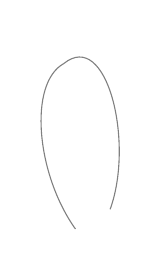
\begin{tikzpicture}[x=1cm,y=1cm]
\draw[thin,gray] (0,0) .. controls (-.5,.7) and (-.6,1.85) .. (-.15,2.1) .. controls (.4,2.55) and (.75,1.1) .. (.44,.25);
\end{tikzpicture}}}

\handwritten{\figure{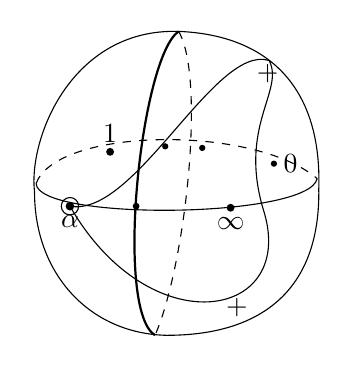
\begin{tikzpicture}[x=1cm,y=1cm]
\draw (0,1.9) .. controls (-1.36,1.94) and (-1.91,.54) .. (-1.83,-.14) .. controls (-1.83,-1.18) and (-1.13,-1.94) .. (-.15,-1.96) .. controls (1.1,-1.96) and (1.8,-1.34) .. (1.78,-.1) .. controls (1.82,1.14) and (1.19,1.85) .. (0,1.9);
\draw[dashed] (-1.81,-.03) .. controls (-1.54,.68) and (.95,.72) .. (1.76,.03);
\draw (1.76,.03) .. controls (1.65,-.48) and (-1.8,-.51) .. (-1.81,-.03);
\draw[thick] (0,1.9) .. controls (-.48,1.57) and (-.82,-1.63) .. (-.3,-1.96);
\draw[dashed] (0,1.9) .. controls (.35,1.3) and (.08,-1.1) .. (-.3,-1.96);
\draw[thin] (-1.38,-.32) .. controls (-.55,-.47) and (.46,1.75) .. (1.15,1.53) .. controls (1.35,1.14) and (.74,.69) .. (1.09,-.41) .. controls (1.48,-1.77) and (-.37,-2.08) .. (-1.38,-.32);
\draw (-1.38,-.32) circle (.11);
\fill (-1.38,-.32) circle (.055) node[below] {$\alpha$};
\fill (-.87,.37) circle (.05) node[above] {$1$};
\fill (1.21,.22) circle (.04) node[right] {$0$};
\fill (.66,-.34) circle (.05) node[below] {$\infty$};
\fill (-.54,-.32) circle (.043); \fill (-.17,.44) circle (.04); \fill (.3,.42) circle (.04);
\node at (1.13,1.36) {$+$}; \node at (.74,-1.61) {$+$};
\end{tikzpicture}}}

\handwritten{$\mathscr T_{0,4}^{+!}\simeq\Pi_{0,3}\deleted{\unsure{\simeq}}$}

\handwritten{\diagram{\begin{tikzcd}[ampersand replacement=\&,column sep=small,row sep=small]
1\arrow[r]\&\Pi_{0,3}\arrow[r]\arrow[d,equal]\&\mathscr T^+_{0,4}\arrow[r]\arrow[d,"\mathrm{cart}"]\&\unsure{\mathfrak S|\mathscr G}_4\arrow[r]\arrow[d,"\mathrm{can}"]\&1\\
1\arrow[r]\&\Pi_{0,3}\arrow[r]\&\mathscr T^+_{0,1}/\pm1\arrow[r]\arrow[d,phantom,sloped,"\simeq"]\&\mathfrak S_3\arrow[r]\arrow[d,phantom,sloped,"\simeq"]\&1\\
\&\&\mathrm{Sl}(2,\mathbb Z)/\pm1\&\mathrm{Sl}(2,\mathbb Z/2\mathbb Z)\&
\end{tikzcd}}}

\handwritten{\diagram{\begin{tikzcd}[ampersand replacement=\&,row sep=small]
\mathscr T^{+\unsure{/|\prime}}_{0,4}\simeq\mathscr T^+_{0,1}/\pm1\arrow[d,phantom,sloped,"\simeq"]\\
\mathrm{Sl}(2,\mathbb Z)/\pm1
\end{tikzcd}}}

\handwritten{\diagram{\begin{tikzcd}[ampersand replacement=\&,column sep=small,row sep=tiny]
0\arrow[r]\&\Pi_{0,3}\arrow[r]\&\mathscr T^+_{0,1}\arrow[r]\arrow[d,equal]\&\deleted{\unsure{\mathbb Z/2\mathbb Z|\mathfrak S}}\widetilde{\mathfrak S}_3\arrow[r,dash]\arrow[d,equal]\&1\\
\deleted{\unsure{e_1,e_2,e_1+e_2|e_1,e_2,e_1,e_2}}\&\&\mathrm{Sl}(2,\mathbb Z)\&\mathrm{Sl}(2,\mathbb Z/4\mathbb Z)/\unsure{---}\&
\end{tikzcd}}}

\handwritten{\diagram{\begin{tikzcd}[ampersand replacement=\&,row sep=small,column sep=small]
\mathrm{Sl}(2,\mathbb Z)/\underbrace{(\pm1.\mathbb Z)}_{\text{\uline{Borel}}}\simeq\&
\unsure{\mathbb P^1(\mathbb Z)|\mathbb P^1_{\mathbb Z}}\arrow[d]\&
{}\simeq\mathbb P^1(\mathbb Q)\\
\&\mathbb P^1(\mathbb Z/2\mathbb Z)\&
\end{tikzcd}}}

\handwritten{$\mathscr T\qquad\Pi_{0,3}$}

\handwritten{\figure{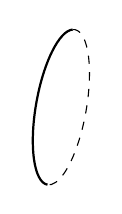
\begin{tikzpicture}
\draw[thick,rotate=-10] (0,0) arc[start angle=-90,end angle=-265,x radius=.32cm,y radius=1cm];
\draw[dashed,rotate=-10] (-.028,1.996) arc[start angle=95,end angle=-90,x radius=.32cm,y radius=1cm];
\end{tikzpicture}}}

\handwritten{$\unsure{\mathfrak{gl}|\mathrm{gl}|\mathrm{Gl}}(2,F_2)$}

\handwritten{\[
\begin{aligned}
&&l_0\,l_1\,l_2\,l_3&=1\\
l_0\,l_1\,l_\infty&=1\\
l'_{\unsure{\infty|0}}\,l'_2\,l'_3&=1&&l_\infty=l'_\infty
\end{aligned}
\]}

\handwritten{\[
\begin{aligned}
&\mathscr T S D\\
&\mathscr T S\qquad\mathscr T D&&\mathbb T S D\\
&\mathscr T&&\mathbb T S\quad\mathbb T D\\
&&&\mathbb T
\end{aligned}
\]}

\handwritten{$\mathscr T_{0,4}^{+\prime}$}

\handwritten{\begin{tabular}{ll}
groupoïdes & $\mathscr T$\\
groupes & $T$\\
multiplicités & $M$\\
\uline{espace} de T & $\widetilde M$
\end{tabular}}

\handwritten{\[
\begin{aligned}
&\mathscr T^+\ \deleted{\unsure{\mathscr T}}\\
&T^+,T^!,T^{+!},\ T^/,T^{/+}
\end{aligned}
\]}

\handwritten{$\mathrm{Gl}(2,\mathbb Z)/\mathbb Z^*$}

\handwritten{\diagram{\begin{tikzcd}[ampersand replacement=\&,column sep=small,row sep=small]
1\arrow[r]\&\unsure{\pi|\Pi}_{g,\nu-1}\arrow[r]\&\mathbb T_{g,\nu}\arrow[r]\arrow[d,phantom,sloped,"\simeq"]\&\underbrace{\mathbb T_{g,\nu-1}}_{X_{g,\nu-1}}\arrow[r]\&1\\
\&\&\pi_1(\mathscr X_{g,\nu-1},\mathbb T_{g,\nu-1};s_\nu)\&\&
\end{tikzcd}}
\[
X_{g,\nu-1}\subset\mathscr X
\]}

\handwritten{\figure{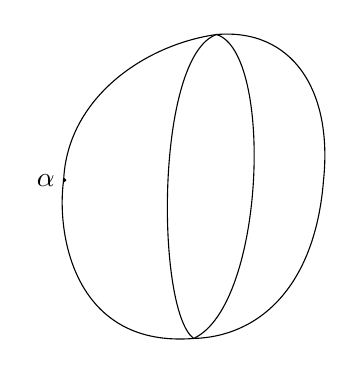
\begin{tikzpicture}
\draw[thin] (0,0) .. controls (-1.5,-.12) and (-1.75,1.3) .. (-1.65,2.02) .. controls (-1.6,3.05) and (-.63,3.73) .. (.29,3.86) .. controls (1.24,3.94) and (1.77,3.17) .. (1.65,2.01) .. controls (1.54,.62) and (.8,.02) .. (0,0);
\draw (0,0) .. controls (-.48,.36) and (-.49,3.58) .. (.29,3.86) .. controls (1.02,3.64) and (.91,.42) .. (0,0);
\fill (-1.64,2.01) circle (.025) node[left] {$\alpha$};
\end{tikzpicture}}}

\handwritten{$\deleted{\unsure{\mathscr M}}M_{g,\nu}\;-$}

\handwritten{$\Pi_{0,3}\qquad\mathfrak S_3$}

\handwritten{\figure{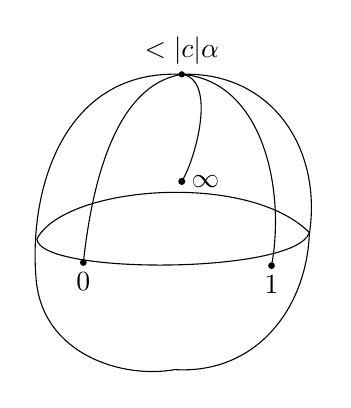
\begin{tikzpicture}
\draw (.12,1.83) .. controls (-1.36,1.9) and (-1.83,.4) .. (-1.73,-.77) .. controls (-1.65,-1.73) and (-.63,-2.04) .. (.03,-1.92) .. controls (1.07,-1.98) and (1.7,-1.14) .. (1.74,-.2) .. controls (1.91,.9) and (1.25,1.87) .. (.12,1.83);
\draw[thin] (-1.72,-.26) .. controls (-1.36,.42) and (.97,.6) .. (1.74,-.18) .. controls (1.57,-.71) and (-1.69,-.72) .. (-1.72,-.26);
\draw (-1.13,-.56) .. controls (-.97,.9) and (-.55,1.72) .. (.12,1.83) .. controls (1.15,1.75) and (1.44,.37) .. (1.26,-.6);
\draw (.12,1.83) .. controls (.57,1.77) and (.3,.76) .. (.12,.47);
\fill (.12,1.83) circle (.04) node[above] {$\unsure{<|c|\alpha}$};
\fill (.12,.47) circle (.045) node[right] {$\infty$};
\fill (-1.13,-.56) circle (.043) node[below] {$0$}; \fill (1.26,-.6) circle (.043) node[below] {$1$};
\end{tikzpicture}}}

% printed form
{\tiny
\begin{verbatim}
//*   CRAY2   0369       I
           00000000      00000000      00000000      00000000
         0000000000    0000000000    0000000000    0000000000
       00      0000  00      0000  00      0000  00      0000
      00     00 00  00     00 00  00     00 00  00     00 00
     00    00  00  00    00  00  00    00  00  00    00  00
    00   00   00  00   00   00  00   00   00  00   00   00
   00  00    00  00  00    00  00  00    00  00  00    00
  00 00     00  00 00     00  00 00     00  00 00     00
 0000      00  0000      00  0000      00  0000      00
000       00  000       00  000       00  000       00
0000000000    0000000000    0000000000    0000000000
00000000      00000000      00000000      00000000

 CCCCCCCCCC   RRRRRRRRRRR    AAAAAAAAAA   YY        YY   2222222222
CCCCCCCCCCCC  RRRRRRRRRRRR  AAAAAAAAAAAA  YY        YY  222222222222
CC        CC  RR        RR  AA        AA   YY      YY   22        22
CC            RR        RR  AA        AA    YY    YY              22
CC            RR        RR  AA        AA     YY  YY               22
CC            RRRRRRRRRRRR  AAAAAAAAAAAA      YYYY               22
CC            RRRRRRRRRRR   AAAAAAAAAAAA       YY              22
CC            RR    RR      AA        AA       YY            22
CC            RR     RR     AA        AA       YY          22
CC        CC  RR      RR    AA        AA       YY        22
CCCCCCCCCCCC  RR       RR   AA        AA       YY       222222222222
 CCCCCCCCCC   RR        RR  AA        AA       YY       222222222222

****A  START  JOB  369  CRAY2                         ROOM        3.45.56 PM 16 AUG 82  R6.PR1    SYS JES2  JOB  369  START  A****
****A  START  JOB  369  CRAY2                         ROOM        3.45.56 PM 16 AUG 82  R6.PR1    SYS JES2  JOB  369  START  A****
****A  START  JOB  369  CRAY2                         ROOM        3.45.56 PM 16 AUG 82  R6.PR1    SYS JES2  JOB  369  START  A****
****A  START  JOB  369  CRAY2                         ROOM        3.45.56 PM 16 AUG 82  R6.PR1    SYS JES2  JOB  369  START  A****
****A  START  JOB  369  CRAY2                         ROOM        3.45.56 PM 16 AUG 82  R6.PR1    SYS JES2  JOB  369  START  A****
****A  START  JOB  369  CRAY2                         ROOM        3.45.56 PM 16 AUG 82  R6.PR1    SYS JES2  JOB  369  START  A****

DERNIERE MISE A JOUR DE JOURNAL : 11-08-82
ATTENTION .............
   ]      1. UNE MODIFICATION SYSTEME NOUS CONTRAINDRA A DETRUIRE
   ]         LE CONTENU DU DISQUE-SPOOL LE MARDI 17 AOUT A 6 HEURES
   ]         VEUILLEZ RECUPERER VOS SORTIES EN ATTENTE AVANT CETTE
   ]         DATE. MERCI DE VOTRE COMPREHENSION.
   ]      2. UN ARRET EXCEPTIONNEL POUR PREPARER L'ARRIVEE DE NOUVELLES
   ]         UNITES AURA LIEU DU VENDREDI 20 AOUT A 17H 30 AU LUNDI
   ]         23 AOUT A 8H.
\end{verbatim}
}

% archive sheet number: 53
